\begin{figure}[H]
	\centering
	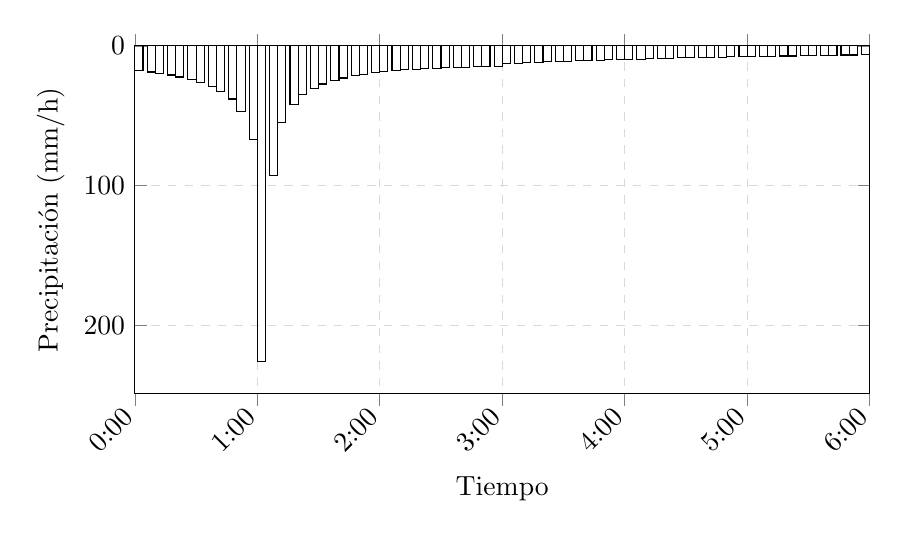
\begin{tikzpicture}
		\begin{axis}[
			width=0.9\textwidth,
			height=6cm,
			xlabel={Tiempo},
			ylabel={Precipitación (mm/h)},
			y dir=reverse,
			ymin=0,
			ymax=249,
			xmin=0,
			xmax=360,
			ybar,
			bar width=4,
			xtick={0, 60, 120, 180, 240, 300, 360},
			xticklabels={0:00, 1:00, 2:00, 3:00, 4:00, 5:00, 6:00},
			xticklabel style={rotate=45, anchor=east},
			grid=major,
			grid style={dashed, gray!30},
			]
			\addplot [
			draw=black,
			fill=none
			]
			coordinates {
				(2, 17.76) (8, 18.72) (12, 19.68) (18, 20.88) (22, 22.32)
				(28, 24.00) (32, 26.16) (38, 28.80) (42, 32.64) (48, 38.04)
				(52, 47.16) (58, 67.20) (62, 226.08) (68, 92.76) (72, 54.84)
				(78, 42.00) (82, 35.04) (88, 30.60) (92, 27.36) (98, 24.96)
				(102, 23.04) (108, 21.48) (112, 20.28) (118, 19.08) (122, 18.24)
				(128, 17.40) (132, 16.92) (138, 16.68) (142, 16.32) (148, 15.96)
				(152, 15.72) (158, 15.48) (162, 15.24) (168, 15.12) (172, 14.88)
				(178, 14.64) (182, 12.72) (188, 12.48) (192, 12.12) (198, 11.88)
				(202, 11.52) (208, 11.28) (212, 11.04) (218, 10.68) (222, 10.56)
				(228, 10.20) (232, 10.08) (238, 9.84) (242, 9.60) (248, 9.48)
				(252, 9.24) (258, 9.00) (262, 9.00) (268, 8.64) (272, 8.52)
				(278, 8.40) (282, 8.28) (288, 8.16) (292, 7.92) (298, 7.80)
				(302, 7.68) (308, 7.56) (312, 7.44) (318, 7.32) (322, 7.32)
				(328, 7.08) (332, 6.96) (338, 6.84) (342, 6.84) (348, 6.60)
				(352, 6.60) (358, 6.48)
			};
		\end{axis}
	\end{tikzpicture}
	\caption{Hietograma - GZ $T_r$=25 años (P=124.7 mm)}
	\label{fig:hyeto_kirpich_gz_Tr25_X125}
\end{figure}
